
\chapter{General Conclusions}\label{chapter6}

We have reported the results of the first studies of the multi-stream environment in cosmological context - from dark matter halo environments to connectivity in single streaming voids. 


\section{Summary of major results}

The full dynamical state of  dark matter can be described as a three-dimensional sub-manifold
in six-dimensional phase space - the dark matter sheet. In our study we use a Lagrangian sub-manifold ${\bf x} = {\bf x}({\bf q},t)$ 
(where {\bf x} and {\bf q} are co-moving Eulerian and Lagrangian coordinates respectively), which 
is dynamically  equivalent to the dark matter sheet but is more convenient for numerical analysis. Counting the number of velocity streams in gravitational collapses supplements our knowledge of spatial clustering. Our major results can be summarized as follows.

\subsection{Heirarchial structure of the dark matter web}

The first study of the multi-stream environment of dark matter haloes in cosmological N-body simulations
in the $\Lambda$CDM cosmology was reported in \cite{Ramachandra2015}. At the resolution of the simulation i.e. without additional smoothing, the cosmic web represents a hierarchical structure: each halo is embedded in the filamentary framework of the web predominantly  at the filament crossings, and each filament is embedded in the wall like fabric of the web at the wall crossings. Locally, each halo or sub-halo is a peak in the number of streams field. The number of streams in the neighbouring filaments is higher than in the neighbouring walls. The walls are regions where number of streams is equal to three or a few. Voids are uniquely defined by the local condition requiring to be a single-stream flow region. We demonstrated in Chapter \ref{chapter3} that the shells of streams around haloes are quite thin and the closest void region is typically within one and a half FOF radius from the center of the halo.

\subsection{Dark matter haloes}

In our simulation reported in Chapter \ref{chapter3}, simple virial density criteria corresponds to a global threshold of $n_{str} \geq 90$ for DM haloes. This shows a reasonably good correspondence with structure finders. A more sophisticated halo finding formulation is done in Chapter \ref{chapter5} assuming that the virialized haloes have convex boundaries. Closed and convex regions of the multistream field are hence isolated by imposing a positivity condition on all three eigenvalues of the Hessian estimated on the smoothed multistream field. In a single-scale analysis of high multistream field resolution and low softening length, the halo substructures with local multistream maxima are isolated as individual halo sites. This halo finding algorithm is free of any heuristic parameters, and maybe extended to delineate filaments, walls, voids, as well as halo sub-structures. 

\subsection{Topological transitions in the web}

Topological connections in the single-streaming voids and multistreaming filaments and walls reveal a cosmic web structure different from traditional mass density fields, as shown in Chapter \ref{chapter4}. A single void structure not only percolates the multistream field in all the directions, but also occupies over 99 per cent of all the single-streaming regions. Sub-grid analyses on scales smaller than simulation resolution reveal tiny pockets of voids that are isolated by membranes of the structure. For the multistreaming excursion sets, the percolating structure is significantly  thinner than the filaments in over-density excursion approach.  
 

\section{Future directions}

Although the scope of this thesis has primarily been multistream field and its application to cosmic structure formation, it is necessary to highlight other important physical quantities derived from the Lagrangian submanifold. For instance, one may track the {\it Flip-Flop} field - a to understand the rich and comples substructures within haloes. On the other hand, Lagrangian submanifold may also be used to identify caustic surfaces -- measure-zero surfaces in the DM Universe that have formally infinite density. 

This section reviews three potential avenues for interesting analyses on Lagrangian submanifold. 

\subsection{Flip-Flop}

The Flip-Flop field, $n_{ff}(\mathbf{q})$ is defined in Lagrangian space by the number of turns experienced by each DM fluid particle. This number is estimated in three dimensions by computing the Jacobian  $J(\mathbf{q}, t) = |\frac{\partial\mathbf{x}}{\partial\mathbf{q}}|$  on each particle at each time step. If the sign of the Jacobian changes, the number of flip-flops for the corresponding particles is increased by one. Details of calculation of flip-flop field and it's significance in understand dynamical history of substructure formation 


\subsection{Caustics}



\subsubsection{Geometric characterization of Caustics}

The inter-particle separation between DM particles in Eulerian space is a generally a good measure of clustering. DM haloes detected by Friends-of-Friends algorithm, for example, are expected to be to have a separation less than 0.2 $\times$ the mean separation of particles in the simulation. Similarly other heuristic thresholds for walls and filaments can be calculated too. 

The DM particles on the caustics are on curved 2-Dimensional surfaces, forming vertices of triangles that constitute the {\it tiles} of the surface. These triangles are of various shapes and size. Since the mean separation of particles is smaller than elsewhere, the triangles are smaller on an average. Figure \ref{fig:PDF_lmax} shows this variation of area of the triangles. Over 8 percent of the triangles have areas less than $10^{-6} h^{-2}Mpc^2$. The distribution function reduces roughly as a power law with the square root of area. 

\begin{figure} 
\centering\includegraphics[width=9cm]{Chapter2/Plots/PDF_triangle.pdf} 
\centering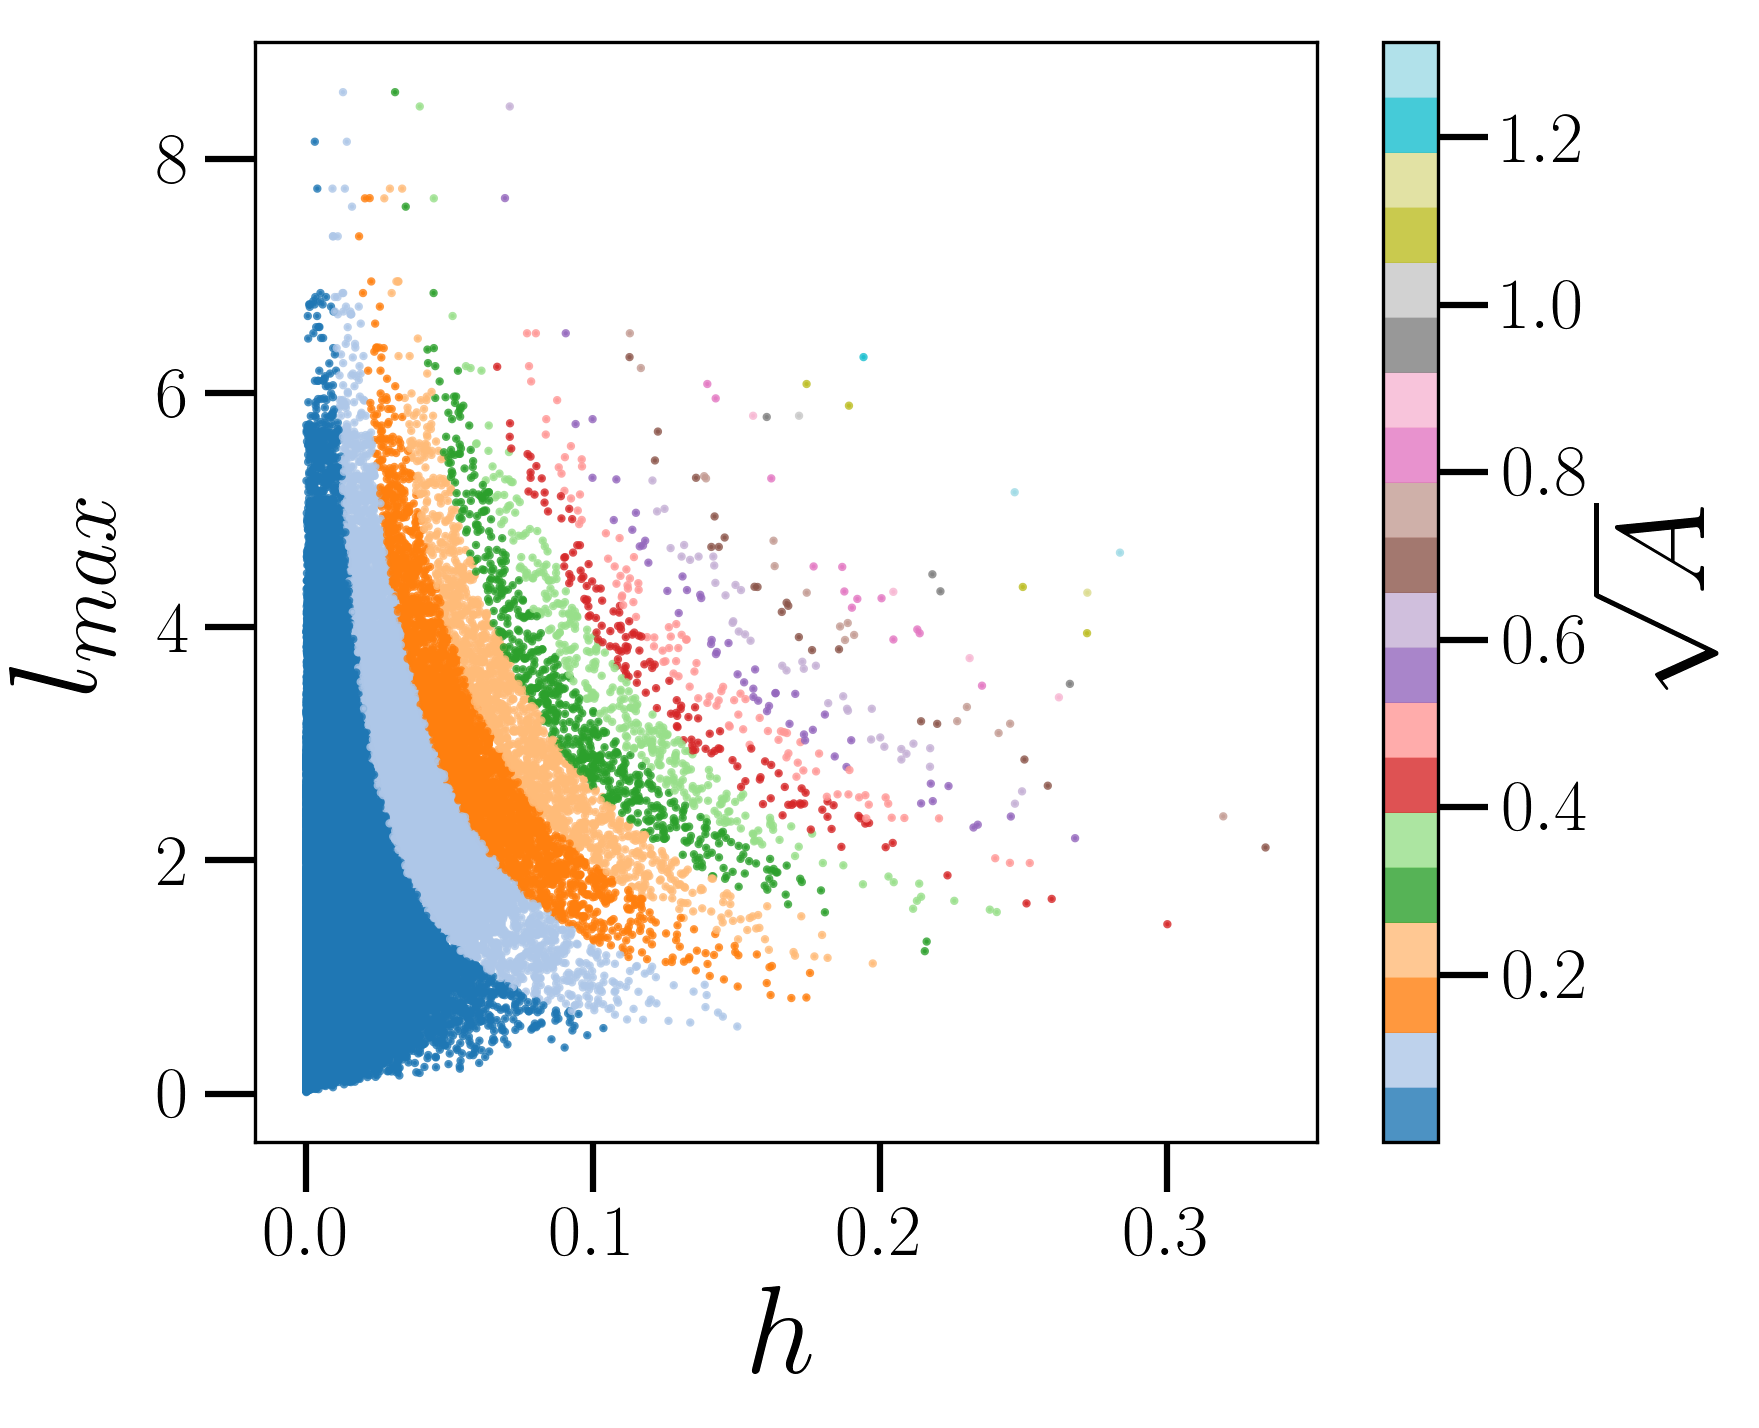
\includegraphics[width=9cm]{Chapter2/Plots/Scatter_Al_ff.png} 
\caption{Top: PDF of triangle discriptors: $l_{max}$ is the largest side of triangles in the caustic surfaces, $h$ is the height, and $\sqrt{A}$ is the square root of area of each triangle. Bottom: Scatter plot of $l_{max}$ and $h$, with $\sqrt{A}$ along the colorbar. }
\label{fig:PDF_lmax}
\end{figure}

However, it was visually seen that several non-compact triangles with small areas were selected. A better heuristic parameter was found to be the longest side of the triangle, $l_{max}$. Choosing this parameter, we circumnavigate the issue of selecting elongated triangles. Variation of $l_{max}$ \hl{is different than that of square root of area} (Figure \ref{fig:PDF_lmax}.)

Finally, using the heuristic parameter of $l_{max}$, we are able to isolate caustic surfaces around specific structures like the haloes. The Figure \ref{fig:caustic_lmax} shows all the caustic surfaces in the top left column, and the inner caustics filtered using $l_{max}$ thresholds in the subsequent coulmns. Furthermore, compared to Figure \ref{fig:caustic_ff}, the inner caustics visually seem to be less elongated. Another interesting aspect of this filtering scheme is the ability to isolate the caustic surfaces around the haloes as seen in the bottom right panel of Figure \ref{fig:caustic_lmax}. 

\begin{figure*} 
\centering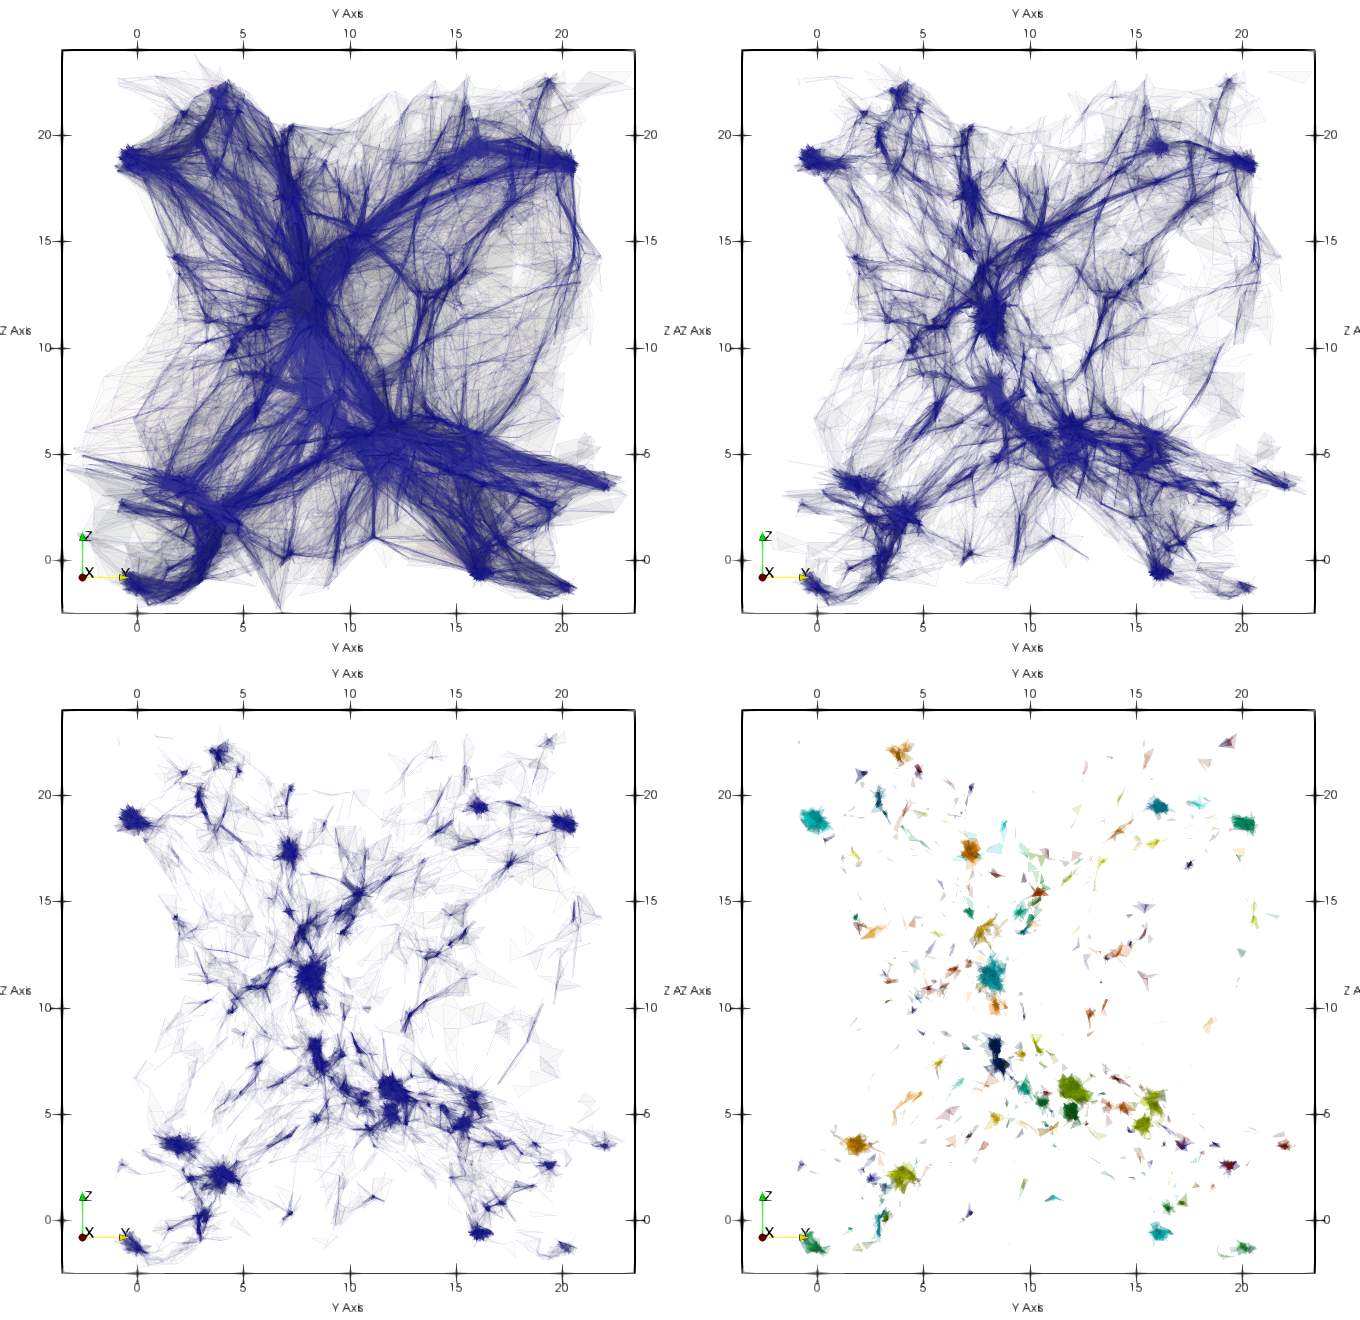
\includegraphics[height=15cm]{Chapter2/Plots/caustic_connectivity.png} 
\caption{$L=20$ Mpc, $N_p = 32^3$. Small simulation, Caustic are filtered by longest side length of the triangle: Top left: $ l_{max} \geq 0$, Top right: $ l_{max} \geq 1$, Bottom left: $ l_{max} \geq 2$, Bottom right: $ l_{max} \geq 3$. }
\label{fig:caustic_lmax}
\end{figure*}


% Combine - caustics and flip-flop to get levels of caustics! However there might be discreetness effects, i.e., say a triangle identified as caustic may have edge particles with 0, 1, 2, 3 .. flip-flops (?). 


% Check this in a small simulation - Run About L = 200/150 Mpc and Np = $32^3$ and pick up highest stream regions - shouldn't be too much. And then see if you can run a zoom-in simulation around halo-site. 

\begin{comment}
\begin{figure} 
\centering\includegraphics[height=15cm]{Plots/percolation.pdf} 
\caption{$L=100$ Mpc (? confirm), $N_p = 128^3$. From Prof. Shandarin - percolation of caustic surface - triangle connectivity is checked. }
\label{fig:1d}
\end{figure}
\end{comment}


Careful examination of the smaller caustic surfaces around the haloes may reveal concentric shells where the particles {\it turn back}. A spherical approximation of this, called the {\it splashback radius} has been analysed by \cite{More2015}. This caustic finding scheme with appropriate filtering is provides a general method to find these boundaries exactly.  

\begin{figure} 
\centering\includegraphics[width=9cm]{Chapter2/Plots/f1fES_caustic.pdf} 
\caption{Percolation in caustic particles with variation of $l_{max}$: Top panel shows the mass fraction of the largest isolated caustic surface $f_1$ and mass fraction of all particles in the caustic $f_{ES}$. Bottom panel shows the filling fraction $f_1/f_{ES}$. Between 3.5-4 $h^{-1} Mpc$ the caustic surfaces transition into distinct isolated surfaces -- i.e., forming turn-around boundaries of haloes. }
\label{fig:f1fES}
\end{figure}



% \subsection{Other avenues}
%  Splashback radii, Merger trees, improvements in simulation etc. 


\section{Final remarks}

%% From Paper2017a intro

Tracing the Lagrangian sub-manifold also provides rich insights into caustics (\cite{Arnold1982} and \citealt{Hidding2014}) and halo collapse \cite{Neyrinck2016}. Recently, there are attempts to improve N-body simulations (see \cite{Hahn2013}, \cite{Angulo2013a}, \cite{Angulo2013b}, \cite{Sousbie2015} and \cite{Hahn2016a}) by solving the Vlasav-Poisson equation using tessellations in the Lagrangian sub-manifold. Galaxy evolution and star formation in the context of multi streaming phenomenon are studied by \cite{Aragon-Calvo2016}. 
